% main2.tex -- H-main.  Section 2: the idea in pictures.
%======================================================================
\section{The idea in pictures}\label{sec:idea}
%======================================================================

Harry's task is to pass within $\varepsilon$ of every point of the front (Figure~\ref{fig:problem}(b)), a closed curve
whose points all run away from him at speed $v$. Our path does this in two acts.

\begin{definition}[Design~T]\label{def:designT}
Let $d=1$ and $t_1:=1/(1-v)+1=2+\mu$.
\begin{itemize}
\setlength{\itemsep}{1pt}\setlength{\parskip}{0pt}
\item \textbf{Run 1:} $P(t):=t$ for $0\le t\le t_1$.
\item \textbf{Run 2:} Let $\alpha_0:=\arccos(v+1/t_1)$ and write $S_{\alpha_0}(t_1)-P(t_1)=\rho_0e^{i\beta^*}$; put
$\hat n:=e^{i\beta^*}$. Set $P(t):=P(t_1)+(t-t_1)\hat n$ for $t_1\le t\le t_\td$, where
\[
t_a:=t_1+\frac{\rho_0-\varepsilon}{1-v},\qquad t_\td:=t_a+\varepsilon\int_0^1\frac{d\sigma}{1-v\sigma(2-\sigma)},
\qquad t_c:=t_1+\frac{\rho_0}{1-v}.
\]
\end{itemize}
\end{definition}

In words: Harry first runs straight through the front and a distance $1$ beyond it, catching direction $0$ on the way.
He then runs straight at the candidate $\alpha_0$, which is chosen so that his line of approach is \emph{tangent} to the
front (at $v=0$ the front is the unit circle and run~2 is the tangent from the point $2$ to $e^{i\pi/3}$). The time
$t_\td$, the \emph{touch-down}, is the moment Harry reaches the regularised version of candidate $\alpha_0$
(Section~\ref{sec:virtual}): $t_a$ is when he arrives within $\varepsilon$ of it, and the integral is the exact time the
remaining distance $\varepsilon$ takes when that candidate flees with the reduced speed of Definition~\ref{def:F}
($t_c$ is when he would meet the true candidate $\alpha_0$; it is used only in Appendix~B). After
touch-down Harry \emph{walks the front}: he repeatedly runs straight at the point of the front an arclength
$\varepsilon$ further along, until he has passed all of it (Definition~\ref{def:chase}). Figure~\ref{fig:designT} shows
the whole path, computed numerically.

\begin{figure}[!htbp]
\centering
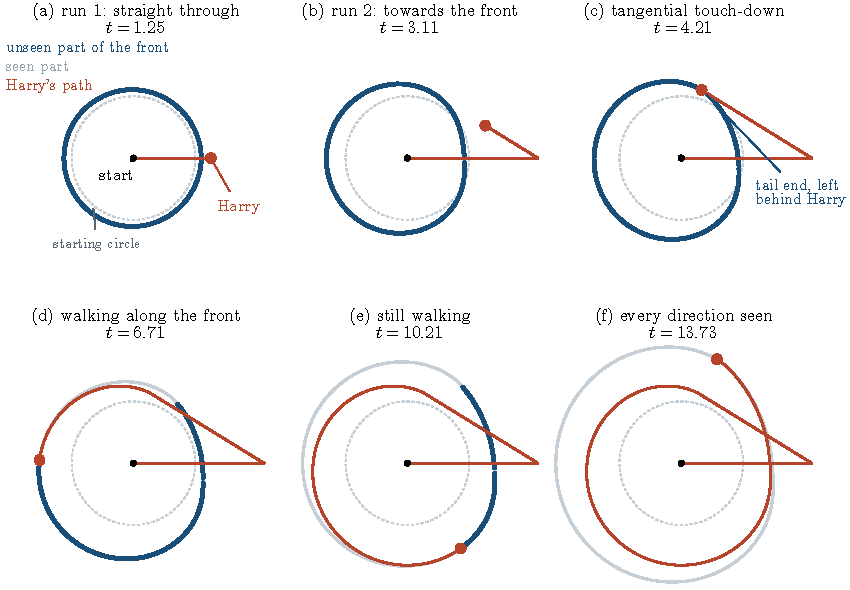
\includegraphics[width=0.98\linewidth]{figs/fig_designT.pdf}
\caption{The path of the proof, simulated for $v=0.1$ and $\varepsilon=0.02$. Harry (red) runs through the front, turns,
touches it tangentially, and then walks along it. The unseen part of the front is dark blue; the seen part fades to
grey. All directions are seen at $t\approx13.7$ (for $v\le v_0$ the proof gives $15$). As $v=0.1$ is not small, the
touch-down point is not $e^{i\pi/3}$ (its $v=0$ position) but about $0.33+1.10i$, at polar angle about $73^\circ$; the
candidate met there has direction $\alpha_0\approx55^\circ$. The simulation walks the whole front of regularised
candidates, including the sliver seen at touch-down and the labels near direction~$0$; the proof cuts that sliver off and
uses true candidates and the point $Z_s$ (Theorem~\ref{thm:touchdown}). So this is a close variant of the path of
Theorem~\ref{thm:main}.}
\label{fig:designT}
\end{figure}

\textbf{Why the walk can take bounded time.} Walking along a nearly straight piece of curve costs about its length, and
each leg sees everything it passes. The front has length about $2\pi$ and, as long as it stays nearly straight near
Harry, it does not grow much during the walk. So the walk should take a bounded time. The danger is \emph{bending at
small scales}: the candidates closest to Harry are pushed in quickly changing directions, and if the front crinkled at
scale $\varepsilon$, every leg would gain little and the walk could take a time growing with $1/\varepsilon$. The proof
must show that the front stays flat at every scale between $\varepsilon$ and a fixed length $R$, uniformly in
$\varepsilon$ --- with constants that do not get worse as $\varepsilon\to0$.

\textbf{Why not simply stop at first contact?} The obvious start is to run straight at the front and begin walking as
soon as some candidate is seen. Near that point the front then has a \emph{corner}: the candidates on either side were
pushed sideways by Harry's approach, so the two sides meet at an angle $2\arcsin v$ away from a straight line. Whichever
side Harry walks first, he leaves the other side behind him, and its end sits right next to his starting point. Harry
then runs away from it, and the exact motion on a straight run (Section~\ref{sec:touchdown}) shows what happens: the
left-behind end bends into a \emph{hook} whose direction keeps turning as one zooms in (Figure~\ref{fig:hook}(a)),
towards the direction perpendicular to Harry's path. On the piece of label length $\delta$ at the end, its relative
bendiness (the average angle between the arc and its chord) decays only like $\delta^{v/(1+v)}$ as $\delta\to0$, far
more slowly than the decay like $\delta^{\gamma}$, $\gamma=\frac23$, that the bootstrap requires
(Section~\ref{sec:virtual}). (Simulations suggest
that Harry still wins from such a start, through a delicate self-correcting balance, but we know no proof of that.)

\begin{figure}[!htbp]
\centering
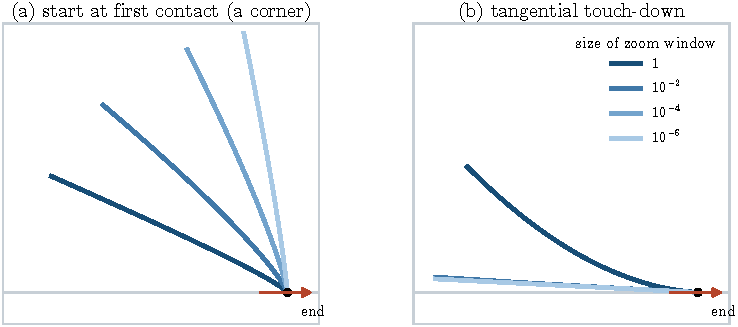
\includegraphics[width=0.92\linewidth]{figs/fig_hook.pdf}
\caption{A \emph{model arm} of the front, left behind by Harry as he runs off to the right, at time $1$ after he leaves
it ($v=0.2$, true candidates, exact straight-run motion). Each curve is the same end, seen through a zoom window of the
indicated size and magnified to unit size. (a) Start at first contact, idealised with $\varepsilon=0$: a straight ray at
the angle $2\arcsin v$ to Harry's backward direction, ending exactly at Harry. The end hooks: the finer the zoom, the
more it has turned (towards the perpendicular of Harry's path). (b) Tangential start: the parabola $y=s^2/2$ tangent to
Harry's path, ending $0.03$ behind him. Its end looks straight at every fine scale (automatic for a curve analytic at
positive distance from Harry; the comparison with (a) concerns $\varepsilon\to0$ with the tail end at distance
$z_0\gg\varepsilon$, as in Theorem~\ref{thm:touchdown}); only at scale $1$ does one see the curvature of the arm.}
\label{fig:hook}
\end{figure}

\textbf{The tangential touch-down.} Design~T avoids the corner. On run~2 Harry grazes the front along a tangent line, so
he sees only a thin sliver of candidates, of length about $\varepsilon^{1/2}$, and the front at touch-down is a smooth
curve tangent to his heading at both of its ends (Figure~\ref{fig:touchdown} in Section~\ref{sec:touchdown}). The end
he leaves behind is again close to him, at distance of order $\varepsilon^{1/2}$, but it is \emph{straight}, pointing
back along his path, and it stays straight while he walks away from it (Figure~\ref{fig:hook}(b),
Theorem~\ref{thm:departure}). The price is a little bookkeeping: pairs of points near that end are ``excused'' from the
bootstrap until Harry has walked a fixed distance $\We$; after that they are far from him and have exactly the starting
data the bootstrap needs.
